\documentclass[twocolumn]{article}
\usepackage{graphicx}
\usepackage{pdfsync}

\title{A two-level, multi-strategy model of memory-based control}

\author{David Reitter \\ Dept. of Psychology \\ Carnegie Mellon University \\ reitter@cmu.edu}
\begin{document}

\maketitle

% Initial analysis:

% plotting four different conditions on a per user basis
% this revealed general learning, even where modulation of the environmental inflow was very high at the end (non-linear decreasing).  There was more variance during the initial than during the late steps.
% Also, I saw that some subjects used a particularly bad strategy - some did not learn at all, some maste systematic errors (like overestimating the changes).

% Notably, linear increases could be modeled well.  Linear decreases not so much.  (cf kalish & griffiths ?)


% I can see that the user's choice is correlated with the tank level:

% library(Hmisc)
% xYplot(I(AmountInTank - Goal) + I(-UserOutFlow+UserInFlow) ~ Time.Step,  data=subset(d, Version=="Non Linear decrease"), nx=F, method=smean.cl.boot, type='b',lty.bands=c(2,2), ylim=c(-15,15))

% d2 <- subset(d, Time.Step>80 & Version=="Non Linear decrease")

% d2 <- subset(d, Time.Step>80 & Version=="Non Linear decrease" & Subject=="t10")

% xYplot( I(AmountInTank) + I(UserOutFlow-UserInFlow) + EnvirInFlow ~ Time.Step,  data=d2, nx=F, method=smean.cl.boot, type='l',lty.bands=c(2,2))

% xYplot( I(UserOutFlow-UserInFlow) + EnvirInFlow ~ Time.Step,  data=d2, nx=F, method=smean.cl.boot, type='l',lty.bands=c(2,2), ylim=c(0,7))


% In the non-linear increase condition, I get very large deviation until about the 70th iteration, but that is only due to subject t33.
%  xYplot(I(AmountInTank - Goal) + I(-UserOutFlow+UserInFlow) ~ Time.Step,  data=subset(d.nl, Subject!='t33' & Version=="Non Linear increase"), nx=F, method=smean.cl.boot, type='b',lty.bands=c(2,2), ylim=c(-15,65))


% # Now, let's take a look at individual subjects.

% ds <- subset(d, Time.Step>80)


\section{Introduction}

Real-time control is a common task to humans, whose performance improves with experience. In this example of such a task, human subjects iteratively control water flow out of a water tank, reacting to a changing, independently determined inflow to the tank.  Thus, the core task is to estimate the development of the inflow from discrete samples; the distribution underlying the inflow is a function of time or iterative steps.  Once the next inflow is estimated, subjects can counteract it by choosing an appropriate outflow valve setting.   In the empirical data available to design the model, the inflow function was manipulated across four conditions, combining linear and non-linear, decreasing and increasing inflow.

The model presented here attempts to bridge the specifics of the experiment that produced the provided data, which involved a learning process and arithmetic decision-making, and real-life control problems, which also involve less discrete, non-arithmetic strategies to react to incremental environmental changes and to correlations of human actions and delayed environmental effects.  I propose a model with two layers: a meta-cognitive level, choosing an optimal \emph{strategy} to address the problem, and a task-specific level, which executes each strategy.


\section{Exploratory Analysis of the Data}
\label{sec:expl-analys-data}


Plotting the data reveals a number of interesting effects.  First, let's look at error in terms of deviation between actual and target water levels and in terms of the chosen outflow compared to the actual inflow.  In my analysis and the model, I will concentrate on only one environmental change variable (EnvirFlow = EnvirInFlow - EnvirOutFlow) and one user-controlled variable (UserFlow = UserInFlow - UserOutFlow).  

The overall error of the user-controlled flow appears to be much greater overall in the non-linear than in the linear condition.  Second, error appears greater during the early phase of the experiment than towards the end.  This observation holds both for the non-linear increasing case, where the rate of change in environmental inflow is high at the beginning, and for the non-linear decreasing case, where the rate of change is greatest at the end.  Thus, there seems to be an effect of practice.

The linear case appears to be an easier task for the subjects.  The plots show the means and a bootstrapped 95\% confidence interval over all subjects except subject t33, which was excluded from the analysis as an outlier.

However, looking only at aggregate data is very deceiving in this case.  Plotting the data separately for each subject reveals that they learned to handle the linear cases extremely well; there is initial error, but then they usually hit the target water level with mathematical precision.  Once or twice per subject, the water level changes for a few steps - often, dramatically.  This causes the impression of an overall, constant variance in the data aggregated across subjects. A good model will approximate the behavior of subjects separately.

A more formal analysis of the data using linear regression showed that the visible parameters (environment inflow, water level) and the resulting precise correction provide a good explanation of the error seen in subject's valve setting.  Specifically, subjects seemed to react to the input equally well in the first and the later parts of each experiment; thus, I do not believe that subjects learn the underlying function  for inflow.  Taking a number of observable variables as predictors in the model, I also examined whether the addition of a subject-specific grouping factor could improve the model fit.  Estimating subject-specific parameters for just the observable variables did not improve the models significantly.  Unsurprisingly, this seems to suggest that a purely linear model with comparatively little dynamical behavior is not a satisfactory level of description for such data.


\section{Modeling the data}
\label{sec:modeling-data}

My initial assumption that this problem was similar to general control problems.  Consider the case of somebody taking a hot shower. Suddenly, the water turns a little colder.  Expecting much colder water, the person cranks up the hot water.  The data presented in this challenge would fit this paradigm quite well, if it wasn't for three observations.  First, the experimental setup suggests entering numbers, i.e. the design requires making discrete decisions at fixed time intervals as opposed to giving a continuous, motor response.  Second, the subject-specific data strongly suggests that most subjects, at least for the linear conditions, acquire the slope of the environmental inflow very quickly, but then apply it very accurately with only minimal deviations.  Third, the design does not introduce noise in the crucial controlled variable (environmental in/outflow) visible to the participant.
These observations suggest that the experimental task is taken as an arithmetic problem rather than as a sensory-motor control problem.

The basic strategy to address this problem is to determine the trend (slope) of the environmental inflow.  This calculation is a primarily symbolic operation; I am not primarily concerned here with the details of how subjects perform the algebraic manipulations involved, other than that they arrive at a result with not perfect, but high reliability.  The second algebraic problem they solve is to add the current water level to the expected trend (to predict the next step), and calculate the necessary inflow/outflow in order to reach the target water level of 4.0.

What would the same problem look like if we were to deal with a classical, sensory-motor control problem?  The inflow trend would have to \emph{estimated} (a subsymbolic operation).  My implementation of this variant estimates the difference between expected water levels (usually 4.0, because outflow is manipulated in order to reach this target) and observed water levels.  It learns the obtained estimate of the inflow as ACT-R chunk.  It then uses Blending (Lebiere, 1998) to retrieve a non-noisy, stable estimate of the time-inflow function and estimates (or calculates) the needed outflow.  In my experiments, such a model had two notable characteristics.  First, it tended to overestimate inflows in an underlying linearly decreasing function, and to underestimate them in an underlying linearly increasing function, because blending uses past experience, and not just the most recent experience.  Second, such a model may deal with non-linear functions worse than the humans do. The strong drop in inflow in the final steps in the non-linear decreasing condition caused the model to vastly overestimate inflow (i.e. not notice the drop), while subjects did better.  However, it appears that the subsymbolic model may account for control problems such as the one presented by Bott \& Heit (2004) or also Kalish, Griffiths \& Lewandowsky (2007), where graphical representations were used for input and output, and where subjects showed a tendency to prefer positive, linear correlations.

A subject-by-subject, exploratory analysis of the data reveals that subjects do adopt different strategies.  Subject t11, for instance, estimates the linearly increasing inflow relatively well without consistently over- or underestimating.  Large deviations occur until approx. step 25, after which the inflow is well estimated and also well compensated.   Subject t26, on the other hand, seems to calculate the inflow trend precisely, making successful corrections from step 5, and miscalculating only once (which leads to short oscillation for just a few steps).  The majority of subjects seem to have chosen this (symbolic) precise method for the linearly increasing task.  For the non-linear example, this solution is less likely to be successful and less commonly seen.  Subjects t29 and t39, for instance, both show regular oscillations throughout the experiment.

As a consequence, I my model implements both strategies: \emph{calculating the trend precisely} and \emph{estimating the trend}.

Thus, the model includes two levels:  a \emph{metacognitive process}, describing the choice of strategy, and \emph{control models}, describing the actual decision-making procedure in each strategy.


\subsection{Cognitive Framework}
\label{sec:cognitive-framework}

I present an end-to-end model of the task, implemented within the theory of ACT-R.  I chose ACT-R in order to have a well-validated framework providing primarily memory function in a combination of symbolic and subsymbolic reasoning. 

The instantiation of the framework used here is provided by ACT-UP, a scalable implementation of ACT-R that allows the modeler to under-specify components of the model, usually because there is no primary evidence and no reasonable intuition about those components\footnote{The model is scalable in as it allows for rapid prototyping of complex models; it is also scalable in terms of its runtime efficiency.  This model calculates about 45 iterations/sec with no optimizations and using a Lisp interpreter.}.  Specifically, I do not specify the exact combination of productions (IF-THEN rules), as their structure is unknown, cannot be validated precisely and does not contribute to the predictions or explanations provided by the model.  (It should be noted, however, that productions may well underlie the model's algorithmic specification.)

The components of ACT-R that contribute to the results of the model are \emph{Base-level learning} and its temporal activation decay; symbolic matching and partial matching in memory retrieval, transient noise ($0.25$) in retrieval, and blending (Lakoff 1987, Wallach\&Lebiere 1999).  I assume knowledge of these mechanisms in my description.


\subsection{Common model - Metacognitive Process}
\label{sec:common-model}


All strategies for this task need to come up with a prediction of the next environment inflow value (EnvInFlow'), resulting in an outflow valve setting of $WaterLevel EnvInFlow' - 4.0$.

An initial set of strategies -- among them useful and incorrect ones -- are defined initially.  I assume that strategies are known to (and developed by) each subject rather explicitly.  Specifically, the strategies are \emph{estimation}, and four kinds of \emph{calculation}, whereas only one form of calculation is appropriate to the task, and the other ones reflect wrong assumptions about the underlying inflow/outflow calculations (for instance, assuming that the given environmental inflow needs to be subtracted from the water level to obtain the next level).

The choice of strategy, determined by the \emph{metacognitive process}, is guided by prior experience.  Each iteration produces a prediction.  This is simple in the given task: we expect the water level to be 4.0 after our new outflow value has been applied.   The model monitors the success experienced after executing a strategy.
It commits to memory, at each iteration, an explicit ACT-R chunk encoding

\begin{itemize}
\item type of strategy (estimating, or arithmetic formula)
\item success criterion
\end{itemize}

The success criterion is defined as the deviation from the target water water level ($4.0$, presently) after using the given type of strategy.

This mechanism learns instance-based knowledge, containing descriptions of the strategy and its utility, skipping over the constant situation (cf., IBLT, Gonzalez, Lerch \& Lebiere 2003).
 
I assume a fixed cost of 2.5 seconds to monitor the strategy.  While I consider delays as underspecified with respect to temporal predictions, they are somewhat relevant to the preference of the model for chunks learned more recently, as activation decays with time.

To choose a strategy, we initiate a memory retrieval, requesting a strategy of any type, with success criterion $0.0$.  ACT-R's partial matching and blending mechanisms retrieve the strategy considered most promising.  Specifically, we calculate a blended chunk for each known strategy.  Blending takes into account prior experience and implies a bias for more recent experiences.  We then retrieve the most-active of the blended strategies; activation follows the ACT-R principles, combining a base-level activation (resulting from the blending process), a partial-matching term (preferring strategies with success criterion closer to $0.0$) and transient noise.   Noise leads to explorative behavior; at the beginning of the task, we find that noise has a stronger effect than towards the end, when activations tend to be more settled.

The strategy retrieval mechanism can be formulated in ACT-UP as follows:

\begin{verbatim}
(best-chunk  
  (loop for s in *strategies* collect  
    (blend (filter-chunks (model-chunks)
                          `(:type strategy 
                            :strategy ,s)) 
         nil ;; no cues
         'strategy ;; return type
         `(:strategy ,s))) ;; retrieval spec
  nil ;; no cues
  `(:success 0.0)) ;; retrieval spec 
\end{verbatim}

(\emph{best-chunk} carries out retrieval, choosing the best of a given set of chunks; \emph{blend} provides those chunks (one for each of the four known strategies).   Blending results in a new chunks, whose numerical features are set to the weighted mean of corresponding values in the blended chunks; single values are weighted by their probability of retrieval, which is determined by $e^{a/t}$  (the numerator of the Boltzmann equation).  $t$ specifies a \emph{temperature} held constant at $0.5$ in my model.

After choosing a valve setting, an additional $6$ seconds are spent waiting for the results, as in the experimental environment.  Empirical timing data was not available for this value.


\subsection{Calculation strategies}
\label{sec:calculation-model}

The calculation strategies remember the last $EnvInFlow_{-1}$ value in a buffer, i.e., the model remembers the value precisely during the next iteration.  Then, calculation is attempted on the basis of the visible new $EnvInFlow$.  Mental arithmetic has been studied and modeled elsewhere (e.g., McCloskey \& Lindemann, 1992, Viscuso, Anderson and Spoehr, 1989, Campbell 2008); I abstract away from the details of the arithmetic operations, primarily for reasons of simplicity, but expect that further variance in the model may be explained by a more detailed model of mental arithmetic.  However, my abstract implementation of the addition and subtraction procedures assumes more reliable addition than subtraction, and more reliable subtraction $A-B$ if $A>B$.  These assumptions follow from predictions of models of cognitive arithmetic (Lebiere 1999).   

The calculation takes 10 seconds in the model.


\subsection{Estimation model}
\label{sec:estimation-model}

Estimation differs from calculation in that exact values are not retained in buffers, but stored in and retrieved from memory.  We store the environmental inflow in memory and retrieve the last stored value (noise may lead to misretrievals).  We then determine the difference between this last stored inflow and the current shown inflow, learning this value in a \emph{trend chunk}.

Environmental inflow and water level are shown on the screen, so the crucial variable to be estimated is the first derivative of the inflow (\emph{trend}).  Each mismatch between expected water level (target level) and actual water level constitutes a sample of the trend.  This is committed to memory as an ACT-R chunk.  The current estimate of the trend is then a blend of previously learned trends:

\begin{verbatim}
(blend (filter-chunks (model-chunks)
                      '(:type trend1)) 
       nil
       'trend)
\end{verbatim}

% {\tt 
% trend-chunks $\Leftarrow$ (filter-chunks (model-chunks)  '(:type trend))
% trend-estimate $\Leftarrow$ (blend expected-trend-chunks :cues nil) }

Initial trend estimates are sampled from a random, uniform distribution ([-10;10]).

The estimation takes 5 seconds in the model. 

% - data shows much more exploration initially in the non-linear cond.
% --> symbolic calculation does not work all the time.




\section{Results}

\subsection{Very Informal Qualitative Analysis}

The model appears to replicate the following properties of the available empirical data (Figures~\ref{li.human}--\ref{nd.model}): Subjects manage to hold water levels around the target; linear functions appear more accurate than non-linear ones; there is an initial phase of high variance; some subjects appear to match the environmental inflow very precisely, but still show the occasional breakout.  (All figures show a 95\% confidence interval obtained by bootstrapping.)

I present plots of the data (before parameter optimization) showing that the model, in principle, succeeds at controlling the water and shows variance distributions similar to the human data.  


\subsection{Parameter fitting}

I optimized a small set of parameters across a grid of plausible values: blending temperature=0.5, duration of wait after setting valve = 8sec,  strategy execution time = 5sec (guess) 10sec (calculation).  The target variable optimized was the correlation of water level means for each time step ($1--100$) across all subjects (correlation $0.78$ for linear increasing, but only $0.24$ for nonlinear decreasing condition).  The optimized parameters differed little from what was estimated informally during model development.

However, I was also interested in replicating the error as it changes over time.  Thus, the error in water level as estimated across blocks of 10 steps for each subject and condition by taking the variance of each 10 data points.  The means of these variances across subjects gives an impression of the overall error made during the different phases of each condition.  As an optimization criterion, I calculated the correlation between these variance means for the subjects and the model (which has generated predictions for a comparable number of subjects).  Again, the best average correlation ($0.42$) across all four conditions occurred at blend temperature=0.5, wait=9sec, strategy execution = 5sec/10sec.


Unfortunately, the model's water level error is very poor for the two non-linear conditions (and very good for the linear conditions).  It is unclear at this point whether there is a lot more variance in the empirical data for the non-linear conditions, which would cause poor superficial model fit.  The exploratory analysis (Figure~\ref{nd.model}) suggests that the model, in principle, makes the right predictions.


\subsection{Other inflow functions and the effect of rate of change}

I evaluated the model with two sinoid functions providing the environment inflow.  
Some experiments with other inflow functions are useful to demonstrate the model's predictions regarding control when non-monotonous environmental functions are observed.  Because the model extrapolates linearly, smoothes estimates and biases them towards the more recent past, it can deal with a sine function quite well.  Occasional breaks are predicted due to miscalculations and misjudgments.   A greater rate of change (smaller periods) in the environmental inflow function will lead to more noise (Figure~\ref{si2.model}).
The model does predict more variance of the water level; variance seems to be correlated to the rate of change: shorter periods lead to more subject error.


\subsection{Oscillations due to delay}

Real-word control problems often suffer from oscillatory behavior.  Take the shower example again: reacting to a bout of cold water, the person will initially overcompensate, and the water ends up being much hotter than desired.  During a few oscillations, water temperature converges to the desired level again.  Similar examples can be made of a weaving car or the well-known phenomenon of pilot-induced oscillations (PIO) in the control of aircraft.  One may hypothesize that unexpected external influences (e.g., road conditions or an aircraft entering ground effect during landing) lead to an overestimation of the effect and an increase the likelihood of such oscillations.  I hypothesize that the delay between control input and observed reaction is a main driver in the production of control oscillations.  Such a delay is given in all of the examples mentioned (shower, aircraft and car, specifically in the case of longer reaction times due to drug-induced incapacitation of the driver, or due to stronger-than-expected inertia of a large vehicle). 

From a cognitive point of view, oscillations are known from decision-making, specifically attitude research (Fink et al. 2002).  There, oscillations occur between different opinions about a subject matter, depending on the evidence that was being reviewed.   They also note that cognitive frameworks tend to come with a level of \emph{inertia} in their choices.  ACT-R is no different, with its retrieval mechanism biased towards the recent past examples rather than just the last choice.  Such inertia leads to oscillations.

Indeed, when presented with a delay, the model predicts considerable oscillations (Figures~\ref{delay.li.model} and \ref{delay.nd.model}.  They are quite regular if only the correct calculation strategy is used (for a lack of noise), but in the final model, these oscillations vary in amplitude.  Indeed, this is what was observed in the attitude data.  Fink et al. (2002):
\begin{quote}"However, the oscillatory trajectories do not look like the trajectories predicted by the simple version of the spatial-spring model discussed earlier.  That model predicted constant periods and amplitudes that either remained constant or got steadily smaller (i.e., were damped).  None of the oscillatory trajectories found showed constant periods.  Moreover, some amplitudes suddenly got larger, and oscillations abruptly ended with no gradual damping." \end{quote}

The model predicts significant oscillations for the case of even a single-step delay; their amplitudes and, to some extent, their periods are irregular.

Humans appear to possess strategies to reduce or nearly eliminate oscillations.  Anything else will be implausible given that control problems (like directional control), even complex ones (like speed control of an aircraft) can be reliably learned.  I have implemented a damping mechanism as an additional metacognitive strategy in the model, whose details I will not describe here given that there is little empirical support for specific damping.  Damping is switched off in the submitted model given that we neither have a basis to fit parameters, nor do we have any indication of how subjects differ in their use of damping.

\subsection{Subject-specific biases}

Subjects will perform differently when calculating (and also estimating); thus they will have developed different a-priori biases for specific strategies (calculate vs. estimate).  For lack of data, I chose to not to randomly sample a subject bias from some estimated distribution; the model starts out with no bias for either strategy.


\subsection{Model Tracing}

The model depends on correlating currently visible outcomes with previously made decisions; disconnecting water levels from the models' chosen valve settings prevents the model from learning from its strategic decisions.  Experiments with model tracing showed that the model appropriately reacted to the experienced inflow, but they show little of the variance distribution attributable to the metacognitive process.


\subsection{Parameter  optimization}

Relevant ACT-R parameters (specifically transient noise and base-level learning delay) were kept at their canonical values.

Model-specific parameters that influence the outcome primarily pertain to the assumed durations of the tasks; longer delays imply lower activations at retrieval, rendering noise relatively more important.  These times were not optimized -- a short-coming of the model.  On the one hand, a model that is developed to fit well should use optimized parameters; on the other hand, such parameters are presumably subject-specific and would, thus, have to be estimated per subject.  



\begin{figure}[p]
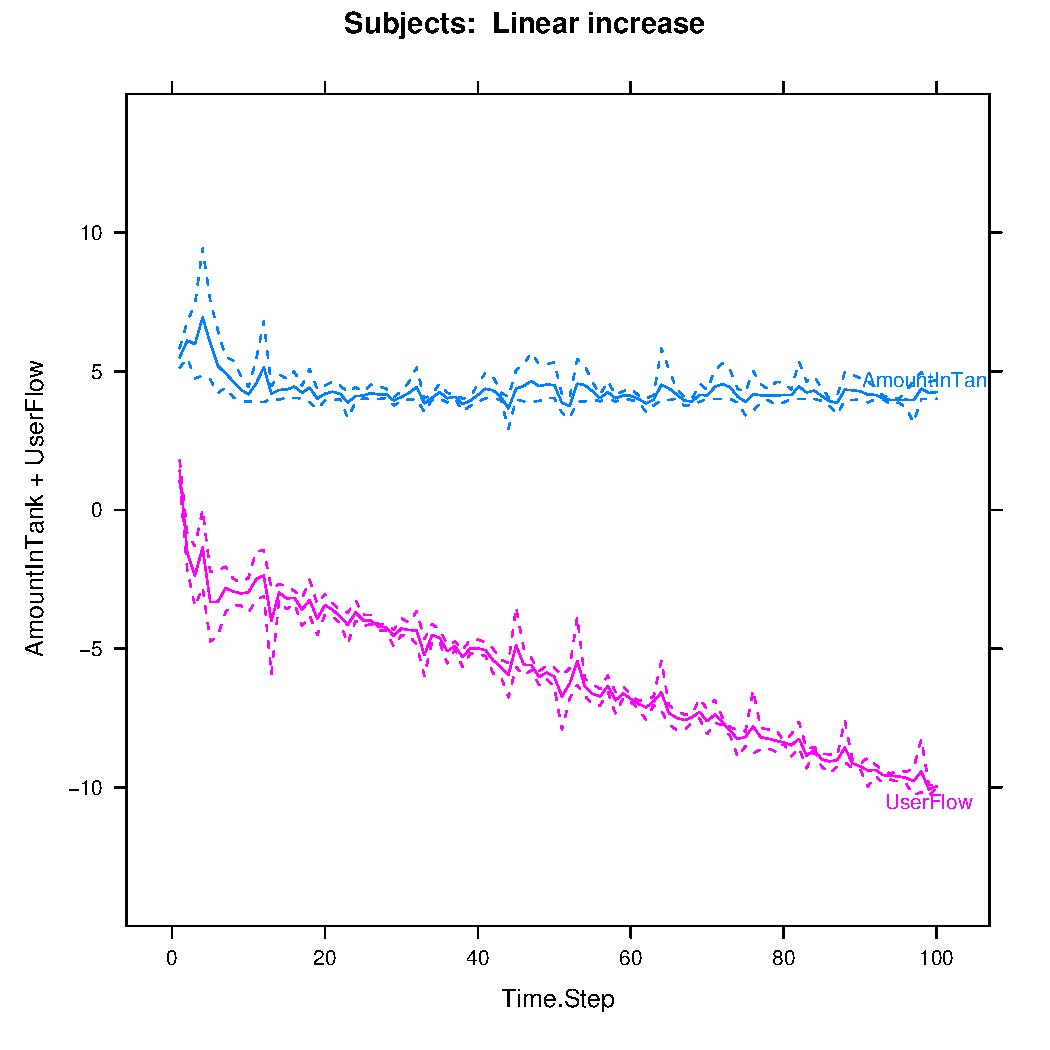
\includegraphics[width=7cm]{li_human.pdf}
\caption{Linear increasing, human data.}
\label{li.human}
\end{figure}
\begin{figure}[p]
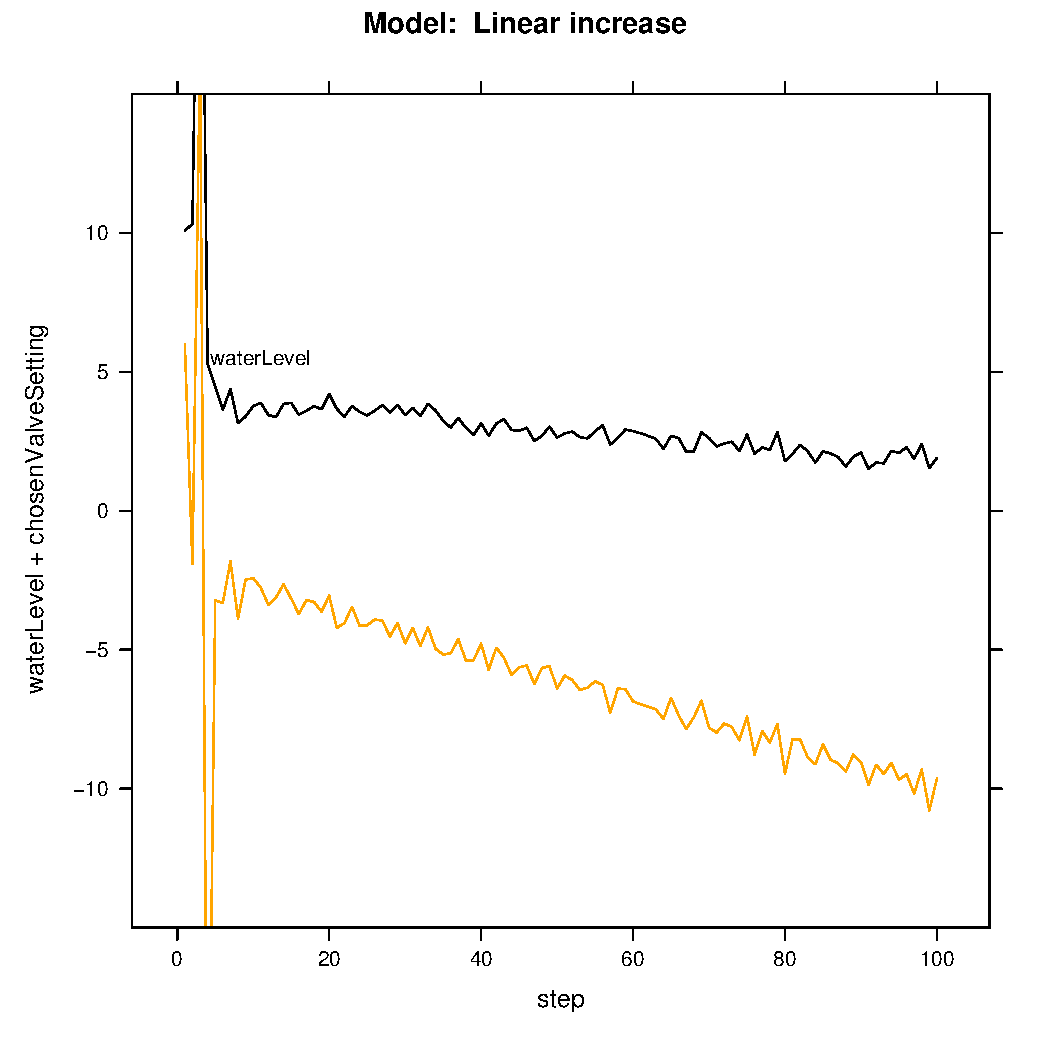
\includegraphics[width=7cm]{li_model.pdf}
\caption{Linear increasing, model.}
\label{li.model}
\end{figure}
\begin{figure}[p]
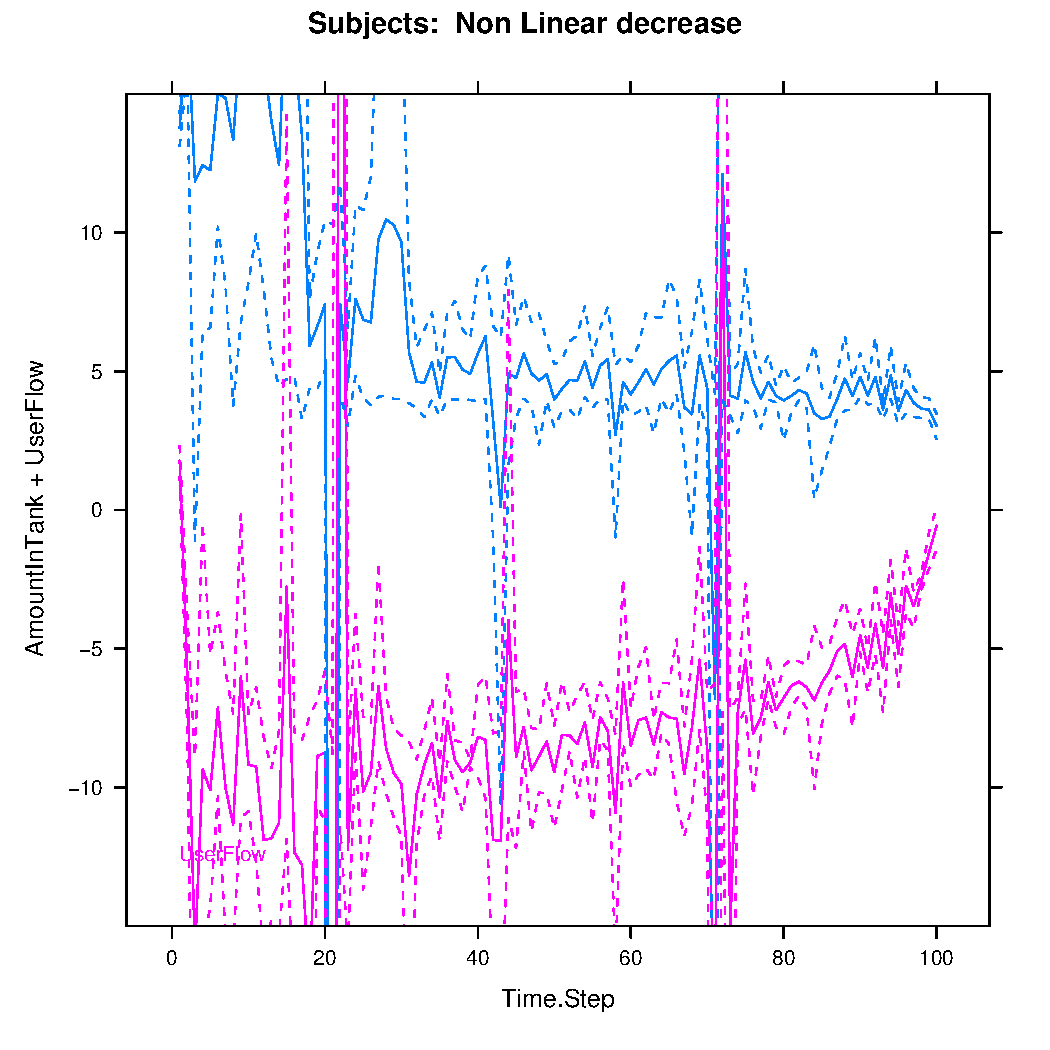
\includegraphics[width=7cm]{nd_human.pdf}
\caption{Non-linear decreasing, human data.}
\label{nd.human}
\end{figure}
\begin{figure}[p]
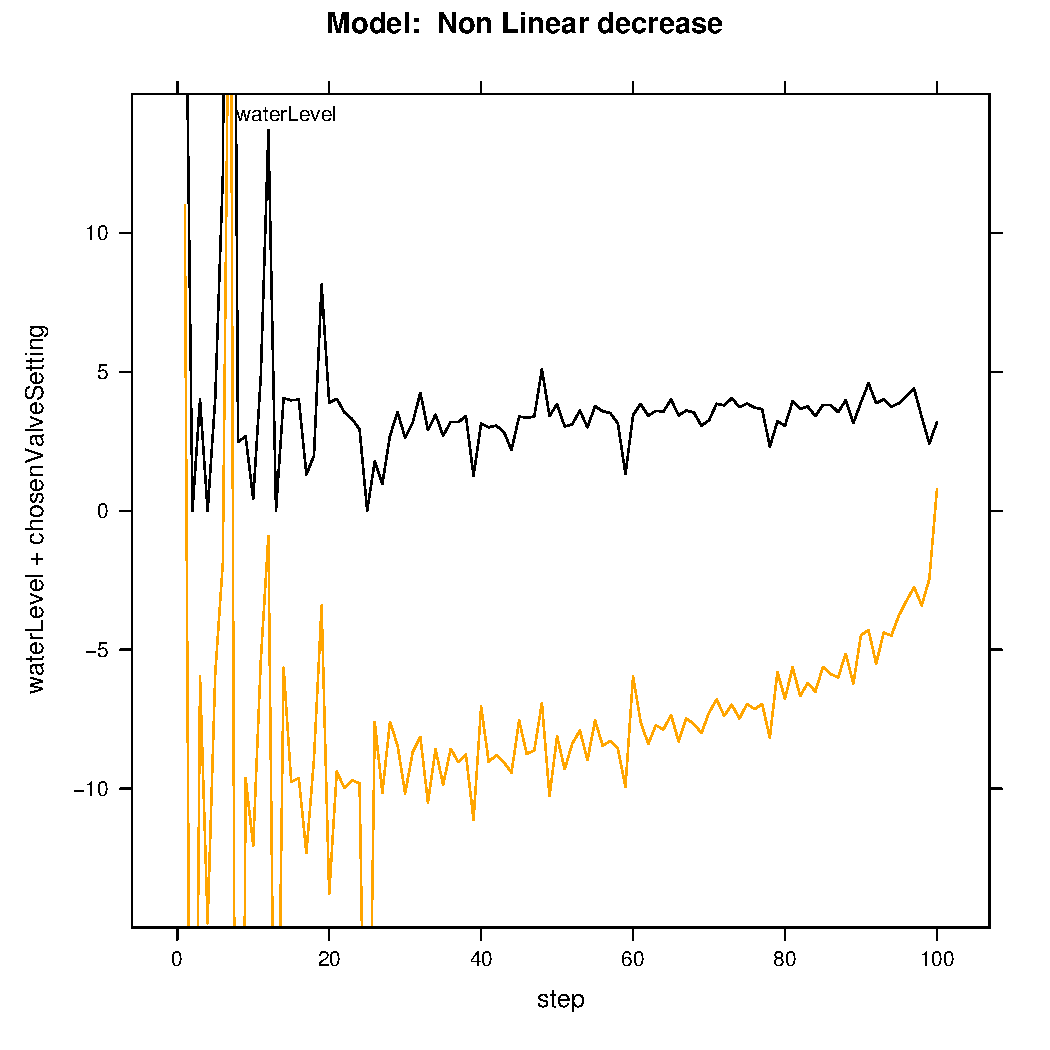
\includegraphics[width=7cm]{nd_model.pdf}
\caption{Non-linear decreasing, model.}
\label{nd.model}
\end{figure}

\begin{figure}[p]
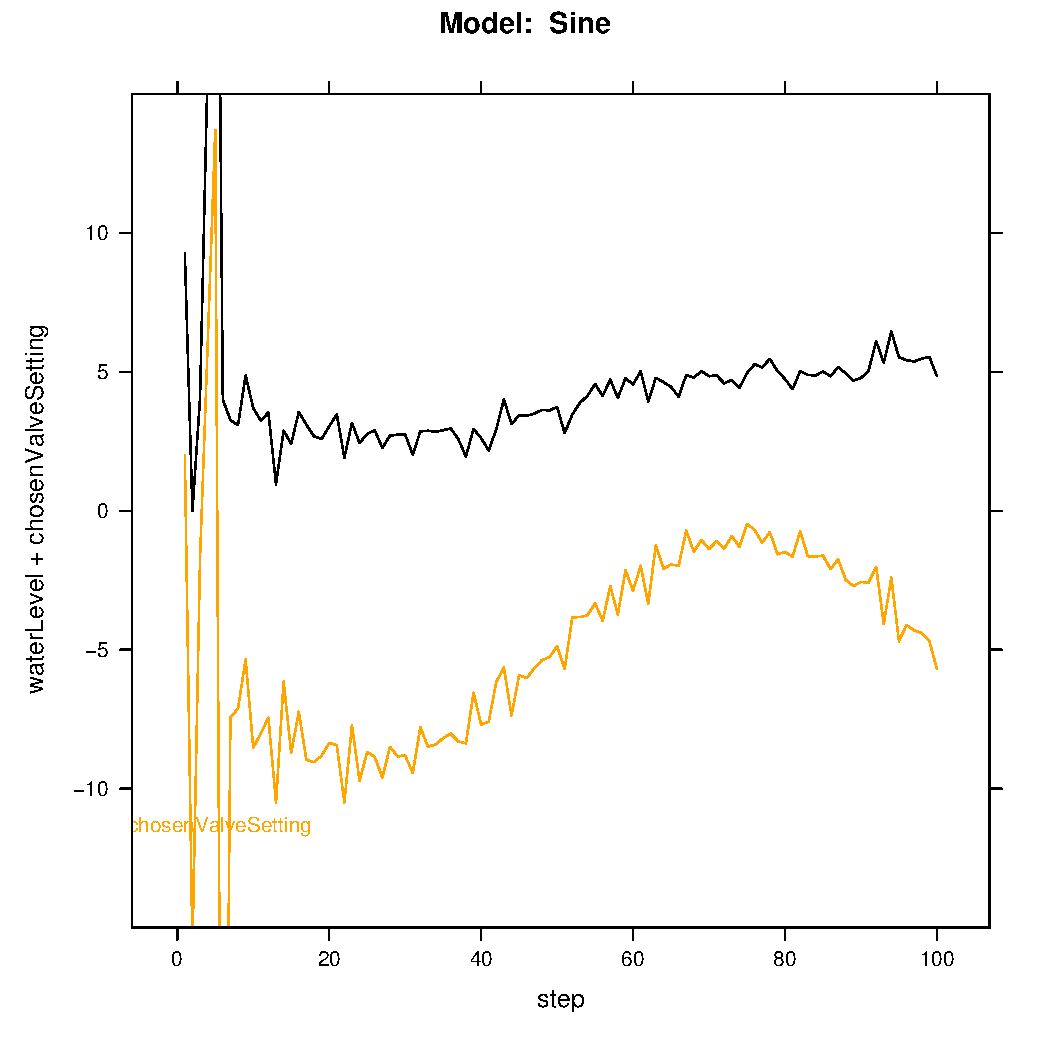
\includegraphics[width=7cm]{sine_model.pdf}
\caption{Sine, model. (Prediction)}
\label{si2.model}
\end{figure}
\begin{figure}[p]
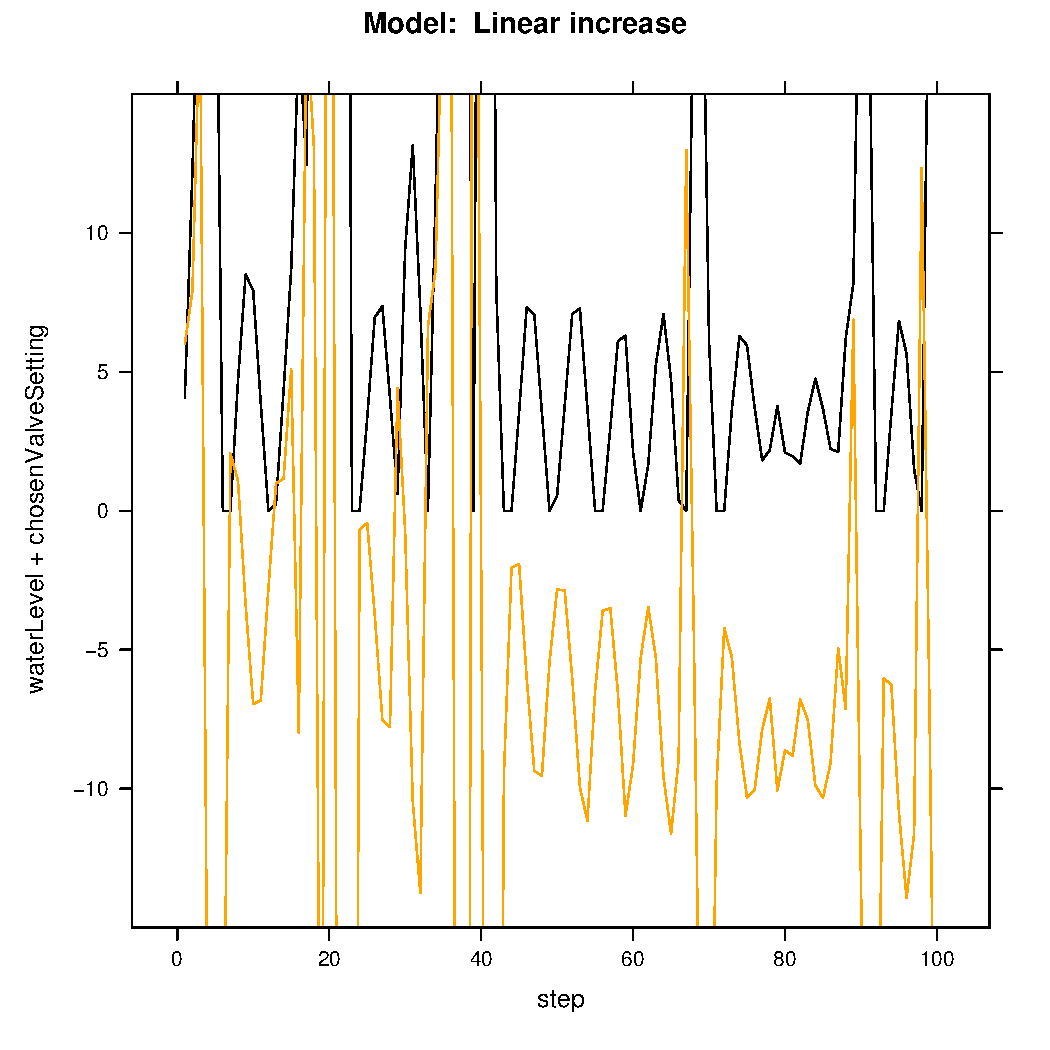
\includegraphics[width=7cm]{li_model_delay.pdf}
\caption{Delay (1 step): Linear increasing, model. (Prediction)}
\label{delay.li.model}
\end{figure}
\begin{figure}[p]
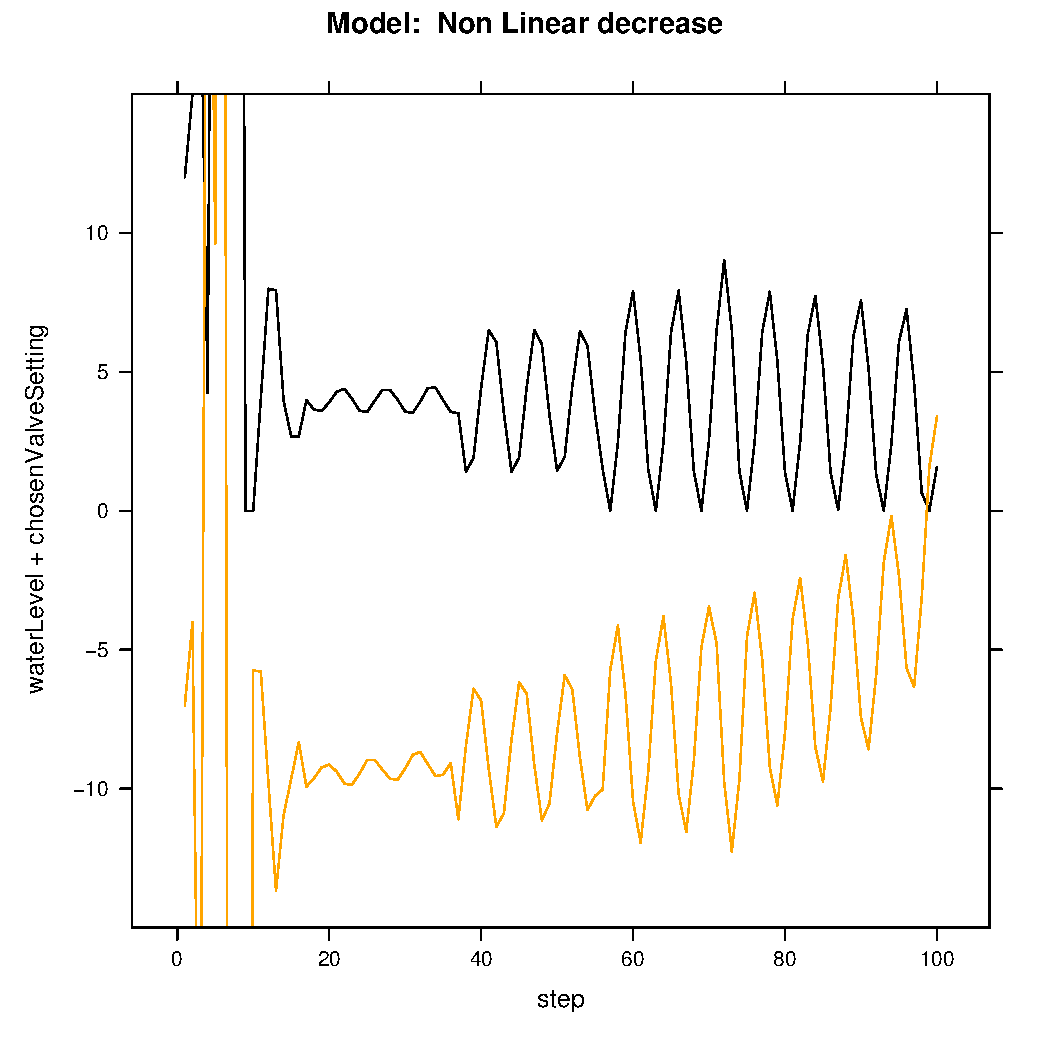
\includegraphics[width=7cm]{nd_model_delay.pdf}
\caption{Delay (1 step): Non-linear decreasing, model. (Prediction)}
\label{delay.nd.model}
\end{figure}

\section*{References}

Fink, E.L., Kaplowitz, S.A., McGreevy Hubbard, S. Oscillation in Beliefs and Decisions. In: Dillard, J.P., Pfau M., The persuasion handbook: developments in theory and practice. Sage, Thousand Oaks CA.

Jamie I. D. Campbell. Subtraction by addition. Mem Cognit 2008 36:1094-1102; doi:10.3758/MC.36.6.1094

Gonzalez, Cleotilde, J. F. Lerch, and C. Lebiere. 2003. Instance-based learning in dynamic decision making. Cognitive Science, 27(4), 591-635. 

Kalish, M. L., Griffiths, T. L., \& Lewandowsky, S. (2007). Iterated learning: Intergenerational knowledge transmission reveals inductive biases. Psychonomic Bulletin and Review, 14, 288-294.

Lebiere, C. (1999). The dynamics of cognition: An ACT-R model of cognitive arithmetic. Kognitionswissenschaft., 8 (1), pp. 5-19
McCloskey M. \& M. Lindemann (1992). MATHNET: preliminary results from a distributed model of arithmetic fact 
retrieval. In Cambpell (edt.) The Nature and Origin of Mathematical Skills. 1992, Elsevier. 

Viscuso, S.R., J.A. Anderson \& K.T. Spoehr (1989). Representing simple arithmetic in neural networks. In (G. 
Tiberghien, edt.), Advances in Cognitive Science Vol.2: Theory and Applications, 144-164. 

Wallach, D., \& Lebiere, C. (1999). Example-based models of control problems. Paper presented at the 1999 ACT-R Workshop, George-Mason University, Fairfax, Va. See http://hfac.gmu.edu/actr99/.



% So, it seems like, at least on the micro-level, tank level seems to be used as input.  We react to it with fairly short delay.


% There is little direct correlation between delta-environment and the user's choices - but they may well be implicit.


% summary(lm( I(-UserOutFlow+UserInFlow)  ~ (EnvirInFlow + I(AmountInTank - Goal)) * Time.Step, data=d.l))
% summary(lm( I(-UserOutFlow+UserInFlow)  ~ (EnvirInFlow + I(AmountInTank - Goal)) * Time.Step, data=subset(d.nl, Subject!='t33' \& Version=="Non Linear increase")))
% summary(lm( I(-UserOutFlow+UserInFlow)  ~ (EnvirInFlow + I(AmountInTank - Goal)) * Time.Step, data=subset(d.nl, Subject!='t33' \& Version=="Non Linear decrease")))
%  summary(lm( I(-UserOutFlow+UserInFlow)  ~ (EnvirInFlow + I(AmountInTank - Goal)) * Time.Step, data=subset(d.l, Subject!='t33' \& Version=="Linear decrease")))
% summary(lm( I(-UserOutFlow+UserInFlow)  ~ (EnvirInFlow + I(AmountInTank - Goal)) * Time.Step, data=subset(d.l, Subject!='t33' \& Version=="Linear increase")))


%  d <- read.csv("/Users/dr/Challenge/human_data.csv", header=T)

% However, it seems like that this is not the basis to estimate subject-specific performance:

% summary(lme( fixed = I(-UserOutFlow+UserInFlow)  ~ (EnvirInFlow + I(AmountInTank - Goal)) + Time.Step, random = ~ ((EnvirInFlow + I(AmountInTank - Goal)) + Time.Step)|Subject, data=subset(d, Subject!='t33')))

% To me, this indicates that (provided the LME fitting algorithm doesnot suffer from lack of data here),  that a linear model does not provide a very meaningful level of description for a cognitive model
% .
% However, it helps us identify relevant parameters.

% Version is predictive of the effect of the parameters:

% lm1 <- lm( I(-UserOutFlow+UserInFlow)  ~ (EnvirInFlow + I(AmountInTank - Goal)) * Time.Step  / Version, data=subset(d, Subject!='t33'))

% best mode so far R^2=0.45

% lme1 <- lme(  I(-UserOutFlow+UserInFlow)  ~ (EnvirInFlow + I(AmountInTank - Goal)) * Time.Step  / Version, random=  ~ Time.Step|Subject, data=subset(d, Subject!='t33'))



 

\end{document}
